\chapter{Branching and Multipass}
\label{c:branch.multi}

\index{branch}
\index{multipass}
The previous chapter (\sref{c:sequence}) covered how to construct a 
lattice branch using \vn{line}s and \vn{list}s. This chapter covers
how to connect the individual branches together to form an entire
accelerator complex. There are two ways this is done. To
describe a fork in an accelerator, \vn{branch} and \vn{photon_branch}
elements may be used. This is described in Section~\sref{s:branching}
With these elements, the connection between a transfer line and a
storage ring or the connection between a storage ring and an X-ray 
line can be simulated.

Branches may also share common elements such as the interaction region
shared by two storage rings. Here a \vn{multipass} line can be used
to describe this. Additionally, \vn{multipass} lines can be used
to describe the case where a beam goes through the same physical
element in a branch multiple times as in an energy recovery linac.
\vn{multipass} lines are described in Section~\sref{s:multipass}.

%-----------------------------------------------------------------------------
\section{Branching with Branch Elements}
\index{photon_branch}\index{branch}
\label{s:branching}

The root branches of a lattice are defined by the \vn{use}
(\sref{s:use}) statement. To further define such things as dump lines,
x-ray beam lines, transfer lines, etc., that branch off from a root
branch, a \vn{branch} or \vn{photon_branch} element (collectively they
can be called branching elements) is used.  \vn{Branch} elements can
define where the particle beam can branch off, say to a beam
dump. \vn{photon_branch} elements can define the source point for
X-ray beams.  Example:
\begin{example}
  erl: line = (..., dump, ...)               ! Define the root branch 
  use, erl
  dump: branch, to = d_line                  ! Define the branch point

  d_line: line = (..., q3d, ...)             ! Define the branch line
\end{example}
The difference between a \vn{branch} element and a \vn{photon_branch}
element is that for a \vn{branch} element the default particle for the
branch is the same as the line that the branch branches off from. The
default particle of the branch from a \vn{photon_branch} element is a
\vn{photon}. The actual particle associated with a branch can be set
by setting the \vn{particle} attribute of the branching element
(\sref{s:branch}).

\index{patch}
Branch lines can themselves have branching elements. A branch line always
starts out tangential to the line it is branching from. The
\vn{direction} attribute of the branch element indicates whether the
branch line is outgoing in the forward direction (direction = +1) or
incoming (direction = -1). A \vn{patch} element (\sref{s:patch}) can
be used at the beginning of a branch line to reorient the reference
orbit as needed.

Like the root branch \bmad always automatically creates an element
with \vn{element index} 0 at the beginning of each branch called
\vn{beginning}. The longitudinal \vn{s} position of an element in a
branch is determined by the distance from the beginning of the branch.

Branch parameters, like whether the branch is open
(``linear_lattice'') or closed (``circular_lattice''), can be set
by setting the appropriate attribute of the \vn{branch} or
\vn{photon_branch} element used to orient the branch.
See \sref{s:branch} for more details.

Branches are named after the branching element name. In the above
example, the branch line would be named \vn{DUMP}. The root branch, by
default, is called after the name in the \vn{use} statement
(\sref{s:use}).

For branch lines (\sref{s:branching}), the ``branch
qualified'' name of an element is of the form
\begin{example}
  branch_name>>element_name
\end{example}
where \vn{branch_name} is the name of the branch and \vn{element_name} is the
``regular'' name of the element. Example:
\begin{example}
  root>>q10w
  xline>>cryst3
\end{example}
When parsing a lattice
file, branches are not formed until the lattice is expanded
(\sref{s:expand}). Therefore an \vn{expand_lattice} statement is
required before branch qualified names can be used in statements. 
See \sref{s:ele.names} for more details.

%-----------------------------------------------------------------------------
\section{Multipass}
\label{s:multipass}
\index{multipass|hyperbf}

Some lattices have the beam recirculating through the same element
multiple times. For example, an Energy Recovery Linac (ERL) will
circulate the beam back through the LINAC part to retrieve the energy
in the beam. In \bmad this situation can simulated using the
\vn{multipass} attribute. A simple example shows how this works.
\index{expand_lattice}
\begin{example}
  A: lcavity
  linac_part: line[multipass] = (A, ...)
  my_line: line = (linac_part, ..., linac_part)
  use, my_line
  expand_lattice
  A\B2[dphi0] = 0.5
\end{example}
The tracking part of the lattice consists of two slave elements
\begin{example}
  A\B1, ..., A\B2, ...
\end{example}
Since the two elements are derived from a \vn{multipass} line they are
given unique names by adding a \vn{{\B}n} suffix. In addition there is
a lord element (that doesn't get tracked through) called \vn{A} in the
lord part of the lattice. Changes to attributes of the lord \vn{A}
element will be passed to the slave elements by \bmad's bookkeeping
routines. Assuming \vn{A\B1} is an accelerating cavity, to make
\vn{A\B2} a decelerating cavity the \vn{dphi0} attribute of
\vn{A\B2} is set to 0.5. This is the one attribute that \bmad's
bookkeeping routines will not touch when transferring attribute values
from \vn{A} to its slaves. Notice that the \vn{dphi0} attribute had to
be set after \vn{expand_lattice} (\sref{s:expand})
is used to expand the lattice since
\bmad does immediate evaluation and \vn{A\B2} does not exist before
the lattice is expanded.

Sublines of a multipass line are automatically multipass:
\begin{example}
  a_line: line = (...)
  m_line: line[multipass] = (..., a_line, ...)
\end{example}
In this example \vn{a_line} is implicitly multipass.

Multiple elements of the same name in a multipass line are considered 
physically distinct:
\begin{example}
  m_line: line[multipass] = (A, A, B)
  u_line: line = (m_line, m_line)
  use, u_line
\end{example}
In this example the tracking part of the lattice is
\begin{example}
  A\B1, A\B1, B\B1, A\B2, A\B2, B\B2
\end{example}
In the control section of the lattice there will be two multipass
lords called \vn{A} and one called \vn{B}. The first \vn{A} lord 
controls the 1\St and 4\Th elements in the tracking part of the lattice 
and the second \vn{A} lord controls the 2\Nd and 5\Th elements.

If a multipass line is reversed then the elements are considered to be
transversed backwards:
\begin{example}
  m_line: line[multipass] = (A, A, B)
  u_line: line = (m_line, -m_line)
  use, u_line
\end{example}
In this example the tracking part of the lattice is
\begin{example}
  A\B1, A\B1, B\B1, B\B2, A\B2, A\B2
\end{example}
Here the 1\St and 6\Th elements are connected to a multipass lord and the
2\Nd and 5\Th elements are connected to a different multipass lord.

%-----------------------------------------------------------------------------
\subsection{The Reference Orbit in a Multipass Line}

\index{lcavity}
\index{p0c}\index{e_tot}
If there are \vn{lcavity} elements in the lattice then the reference
energy at a given element may differ from pass to pass. In this case,
the normalized strength (k1, kick, etc.) for magnetic and electric
elements will not be the same from pass to pass. To avoid an
ambiguity, all magnetic and electric elements that are used in a
multipass line must have their magnetic or electric field strength set
as the independent attribute (\sref{s:depend}), {\em or} a reference
energy (\sref{s:energy}) must be defined. A reference energy is
defined by setting \vn{e_tot} or \vn{p0c}, or by setting
\vn{n_ref_pass} as described below. The default is for \vn{n_ref_pass}
to be set to 1.

\begin{figure}[tb]
\centering 
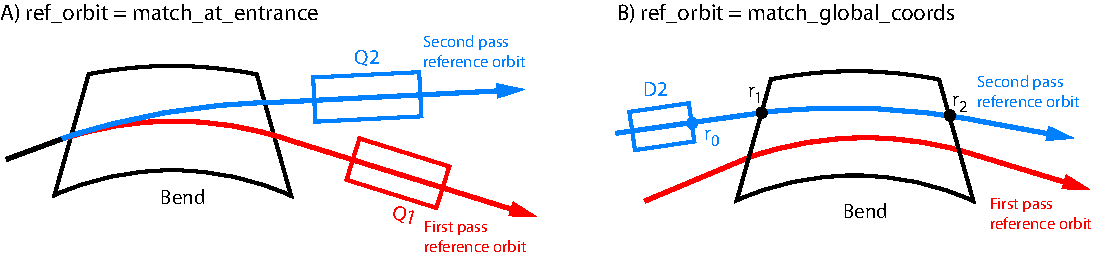
\includegraphics[width=6.2in]{multipass_bend.pdf} 
\caption[The reference orbit with a multipass bend.]  
{A) With \vn{ref_orbit} = \vn{match_at_entrance}, the reference orbits
of different pass will be taken to be the same at the entrance end of
the magnet. If there is a difference in the reference energy through a
bend from pass to pass, the reference orbit through the bend will vary
from pass to pass. B) With \vn{ref_orbit} = \vn{match_global_coords},
the reference orbit on the first pass establishes the position of the
bend in the global coordinate system and the reference orbit on other
passes is calculated with respect to this.}
\label{f:multipass.bend}
\end{figure}

\index{sbend}\index{rbend}\index{patch}
For a bend in a multipass line, there is the added complication of how
to define the reference orbit when the reference energy is different
from pass to pass. If, say, a different reference orbit is used for
each pass there is a problem of how to interpret multipole values like
\vn{k1}. On the other hand, it is sometimes very convenient to be able
to use separate reference orbits. For this reason, a bend element has
a \vn{ref_orbit} attribute that, when combined with the reference
energy, define the reference orbit. \vn{ref_orbit} is a switch that
can take the values:
\begin{example}
  single_ref            ! Default. 
  match_global_coords   ! Must be used with n_ref_pass = 1
  match_at_entrance
  match_at_exit
  patch_in              ! Used with patch elements,
  patch_out             !   and must be used with n_ref_pass = 1.
\end{example}
A value of \vn{single_ref} (the default) means that the {\em same}
reference orbit will be used for all passes. The \vn{match_global_coords},
\vn{match_at_entrance} and \vn{match_at_exit} values are used when
{\em separate} reference orbits are desired as described below.

To set the reference energy, one (and only one) of the attributes
\vn{n_ref_pass}, \vn{e_tot} or \vn{p0c} needs to be
set. \vn{n_ref_pass} is an integer indicating which pass is used to
define the reference energy for the lord element. The default if
nothing is set, is for \vn{n_ref_pass} to be set to 1.  Note: If
\vn{ref_orbit} is set to \vn{match_global_coords}, or for any element
where the reference energy is not constant (like an \vn{lcavity}),
\vn{n_ref_pass} must be used and must be set to 1.

An example will make this clear. Consider a bend defined by
\begin{example} 
  B: sbend, l = 1, b_field = 1.0, n_ref_pass = 1, ref_orbit = single_ref
\end{example}
Here the same reference orbit will be used for all passes. Assume that
the reference momentum \vn{p0c} on the first pass is 5~GeV (this is
determined by the reference momentum at the beginning of the lattice
and any \vn{lcavity} elements in the lattice). Since \vn{n_ref_pass}
is one, this fixes the momentum at which the reference orbit is
calculated to be 5~GeV. The bending radius \vn{rho} of the reference
orbit is related to the field and momentum by
\begin{example}
  rho = p0c / (c_light * b_field)
\end{example}
In this case, this translates into a bending radius of 16.7~m. In the
tracking lattice, the first pass element \vn{B\B1} will have a value
for \vn{b_field} of 1~Tesla just like its lord element. Also,
like its lord element, \vn{B\B1} will have an error field,
\vn{b_field_err}, of zero. The total field
\begin{example}
  b_field_tot = b_field + b_field_err
\end{example}
will be 1~Tesla. Additionally, the edge face angles \vn{e1} and
\vn{e2} will be the same as \vn{B}. In this example both are
zero. This is true for all passes.

Now assume that on the second pass, the reference momentum is 10~GeV.
Since, on the second pass, \vn{p0c} is a factor of 2 larger, to keep
the bending radius invariant, the value of \vn{b_field} for the second
pass element \vn{B\B2} will be a factor of 2 larger. That is, it will
be 2~Tesla. However, the total field in the element must be the
same on all passes (\vn{B\B1} and \vn{B\B2} represent the same
physical element after all). Thus, \vn{B\B2} must have a value for
\vn{b_field_err} of -1~Tesla.

Consider the case where the value of
\vn{ref_orbit} is set to \vn{match_at_entrance} and the reference
momentum is set instead of \vn{n_ref_pass}:
\begin{example} 
  B: sbend, l = 1, b_field = 1.0, p0c = 5e9, ref_orbit = match_at_entrance
\end{example}
Here the reference orbit will be different on the two passes. The two
reference orbits will coincide at the entrance edge of the magnet.
This is illustrated in \fig{f:multipass.bend}A. For both
\vn{B\B1} and \vn{B\B2}, the value of \vn{b_field} will be 1~Tesla
giving bending radii of \vn{16.7}~m and \vn{33.4}~m respectively. With
\vn{B\B2}, the element length will be a slight bit larger than
\vn{B\B1} with a value of \vn{1.0000045}. The entrance face angle
\vn{e1} will always be the same on all passes (zero in this example)
but \vn{e2} will vary. In this case \vn{e2} for \vn{B\B2} will be
\vn{0.003}. With the different reference orbit for the second pass,
there is no good way to handle a non-zero multipole attribute so \bmad
disallows them in this case.

\vn{match_at_exit} is similar to \vn{match_at_entrance} except that
the different reference orbits will coincide at the exit edge of the
magnet. If \vn{match_at_exit} is used with the parameters in the above
example, the only change for \vn{B\B2} is that \vn{e1} will now be
\vn{0.003} and \vn{e2} will be zero.

The \vn{match_at_entrance} value for \vn{ref_orbit} is useful
for simulating a bend at the end of a multipass line that is used to
separate the beams on the various passes. Notice that the next
elements downstream (labeled \vn{Q1} and \vn{Q2} in
\fig{f:multipass.bend}A) will be physically separated in
space. That is, it does not make sense to use \vn{match_at_entrance}
for a bend that is {\em not} at the end of a multipass
line. Similarly, the \vn{match_at_exit} value is useful for simulating
a bend that combines beams of different energies. Such a bend should
be placed at the beginning of a multipass line.

With \vn{ref_orbit} set to \vn{match_global_coords}, the reference
orbit on a given pass is determined by the global coordinates
(\sref{s:global}) of the reference trajectory. Example:
\begin{example} 
  B: sbend, l = 1, b_field = 1.0, n_ref_pass = 1, ref_orbit = match_global_coords
\end{example}
As will be explained, when using \vn{match_global_coords},
\vn{n_ref_pass} must be present and set to 1. With
\vn{match_global_coords}, \vn{B\B1} will have the same parameters as
\vn{B} and this will determine the reference orbit for \vn{B\B1}. See
\fig{f:multipass.bend}B). For the second pass, the reference
trajectory at the entrance end of the bend is determined as follows:
The calculation starts with the global coordinates of the reference
orbit at the exit end of the element just before \vn{B\B2} (marked
$r_0$ in \fig{f:multipass.bend}B)). To be physically correct,
this point must lie on the entrance face of \vn{B\B2}. However, it is
possible to have a lattice where this is not so and the calculation
does not demand this. If $r_0$ does not lie on the entrance face, the
reference orbit is extended (either forward or backward) in a straight
line to a point where it intersects the entrance face (marked $r_1$ in
\fig{f:multipass.bend}B)). The reference radius of curvature is
calculated by scaling the radius as calculated from the first pass
scaled by the change in reference momentum between the first and
second passes. From the entrance point and the radius of curvature,
the exit point (marked $r_1$ in \fig{f:multipass.bend}B)) can
be calculated. The curve from $r_1$ to $r_2$ defines the reference
trajectory through \vn{B\B2}. The face angles \vn{e1} and \vn{e2}, and
the path length \vn{l} for \vn{B\B2} can be calculated from the
geometry.

Since the calculation with \vn{match_global_coords} is rather
complicated, the use of \vn{match_global_coords} is restricted to
lattices that lie horizontally in the global $X-Z$ plane. Also, the
restriction to \vn{n_ref_pass = 1} is necessary since the calculation
becomes nondeterministic otherwise. 

\index{match_at_entrance}\index{match_at_exit}\index{match_global_coords}
\index{sbend}\index{rbend}
Additionally, for a bend, with \vn{ref_orbit} set to either
\begin{example}
  match_at_entrance,
  match_at_exit, or
  match_global_coords
\end{example}
the bend must be a pure dipole. That is, no quadrupole or higher order
components. This assumption is necessary since the reference orbit
calculation assumes that the orbit within the bend is circular for all
reference orbits.

%-----------------------------------------------------------------------------
\subsection{Using Patch elements to Vary the Reference Orbit in a Multipass Line}
\label{s:multi.patch}

\begin{figure}[tb]
\centering 
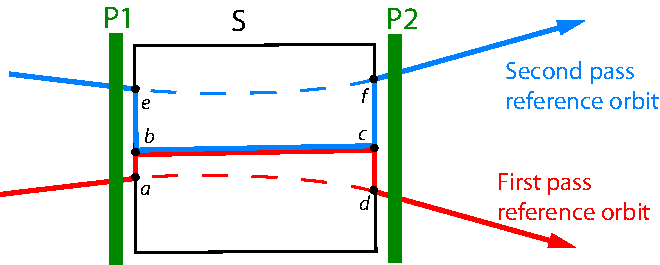
\includegraphics[width=4in]{multipass_patch.pdf} 
\caption[Using patch elements to vary the reference orbit in a multipass line.]
{Using patch elements to vary the reference orbit in a multipass line. 
The gap between \vn{patch} elements \vn{P1} and \vn{P2} and the lattice section 
\vn{S} is for illustration purposes only.
}
\label{f:multipass.patch}
\end{figure}

There exist situations where it is desirable to have different
reference orbits for each pass through a non-bend elements. Such a
situation is illustrated in \fig{f:multipass.patch}. In this
example, beams of differing energy pass through a section of the
lattice labeled \vn{S}. This section may contain one or more
elements. The desired reference orbit for each pass follows the beam
trajectories. This is achieved by placing patch elements, called
\vn{P1} and \vn{P2}, just before and just after \vn{S}. The
corresponding lattice file would look like
\begin{example}
  p1: patch, ref_orbit = patch_in, n_ref_pass = 1, translate_after = True
  p2: patch, ref_orbit = patch_out, n_ref_pass = 1, ref_patch = p1

  m_line: line[multipass] = (p1, S, p2)
  all_line: line = (..., m_line, ..., m_line, ...)
  use, all_line
  
  expand_lattice
  p1\B1[x_offset] = 0.05
  p1\B1[x_pitch] = -0.0034
\end{example}
The \vn{ref_orbit} parameter for \vn{p1} and \vn{p2} indicate whether
the patch is just before (\vn{patch_in}) or just after
(\vn{patch_out}) the section of interest. In this example,
\vn{x_offset} and \vn{x_pitch} parameters for the first pass slave
\vn{p1\B1} are set in the lattice file. This determines the
orientation of the reference orbit through \vn{S} (labeled $b$-$c$ in
the figure) with respect to the incoming first pass reference
orbit. Point $a$ in the figure is the first pass reference orbit just
before \vn{p1\B1} and point $b$ is the reference orbit just after. On
the second pass, \bmad will calculate the patch parameters for
\vn{p1\B2} so that the global coordinates of the reference orbit just
after \vn{p1\B2} is the same as the reference orbit just after
\vn{p1\B1}. That is, point $b$.

The patch parameters for the \vn{p2\B1} first pass slave of \vn{p2},
which has \vn{ref_orbit} set to \vn{patch_out}, the calculation is as
follows: In the definition of \vn{p2} the \vn{ref_patch} parameter is
set to \vn{p1}. \bmad uses this as the starting point for
tracking. \bmad starts with a particle on the reference trajectory
just {\em before} \vn{p1\B1} and tracks it to the end of \vn{S} (curve
$a$-$d$ in the figure). \bmad then sets the parameters of \vn{p2\B1}
so that the reference orbit after the patch (point $d$) coincides
with the particle. The calculation of the second pass slave \vn{p2\B2}
is analogously computed.

The above procedure of defining the reference orbit using patches with
\vn{ref_orbit} set to \vn{patch_in} and \vn{patch_out} is helpful in
designing lattices. However, once a lattice is designed, there will be
a problem for simulations of lattice errors since particle
trajectories, and hence the reference orbit, will be affected by such
errors. To avoid this, once the layout of the lattice has been settled
on, the \vn{patch_in} and \vn{patch_out} patches should be removed and
four new patches, to replace the four multipass slave patches, should
be introduced outside of the multipass section with the patch
parameters set to the appropriate values.
